\documentclass[12pt, titlepage]{article}

\usepackage{booktabs}
\usepackage{tabularx}
\usepackage{hyperref}
\hypersetup{
    colorlinks,
    citecolor=black,
    filecolor=black,
    linkcolor=red,
    urlcolor=blue
}
\usepackage[round]{natbib}
\usepackage{adjustbox}
\usepackage[dvipsnames]{xcolor}
\usepackage{float}
\usepackage{changepage}
\usepackage{pdflscape}

%% Comments

\usepackage{color}

\newif\ifcomments\commentstrue %displays comments
%\newif\ifcomments\commentsfalse %so that comments do not display

\ifcomments
\newcommand{\authornote}[3]{\textcolor{#1}{[#3 ---#2]}}
\newcommand{\todo}[1]{\textcolor{red}{[TODO: #1]}}
\else
\newcommand{\authornote}[3]{}
\newcommand{\todo}[1]{}
\fi

\newcommand{\wss}[1]{\authornote{blue}{SS}{#1}} 
\newcommand{\plt}[1]{\authornote{magenta}{TPLT}{#1}} %For explanation of the template
\newcommand{\an}[1]{\authornote{cyan}{Author}{#1}}

%% Common Parts

\newcommand{\progname}{ProgName} % PUT YOUR PROGRAM NAME HERE
\newcommand{\authname}{Team \#, Team Name
\\ Student 1 name
\\ Student 2 name
\\ Student 3 name
\\ Student 4 name} % AUTHOR NAMES                  

\usepackage{hyperref}
    \hypersetup{colorlinks=true, linkcolor=blue, citecolor=blue, filecolor=blue,
                urlcolor=blue, unicode=false}
    \urlstyle{same}
                                


\begin{document}

\title{Verification and Validation Report: \progname} 
\author{\authname}
\date{\today}
	
\maketitle

\pagenumbering{roman}

\section{Revision History}

\begin{tabularx}{\textwidth}{p{3cm}p{2cm}X}
\toprule {\bf Date} & {\bf Version} & {\bf Notes}\\
\midrule
06/03/2023 & 1.0 & Recorded the results of some functional and non-functional tests\\
08/03/2023 & 1.0 & Finished first version\\
03/04/2023 & 1.1 & Addressed GitHub issues\\
05/04/2023 & 2.0 & Finished second version\\
\bottomrule
\end{tabularx}

~\newpage

\tableofcontents

\listoftables %if appropriate

\listoffigures %if appropriate

\newpage

\pagenumbering{arabic}

This document describes the test results of the verification and validation (VnV) plan for Farming Matters. The VnV plan was continuously updated as the project evolved. The following document records the results of the current version of the VnV plan. It provides results of functional and nonfunctional requirements tests, unit tests, changes that will be implemented in the system as a result of the tests, and various traceability tables.


\section{Functional Requirements Evaluation}

The following section outlines the results of functional testing. The process and test performed follow the VnV Plan. To summarize, all the functional tests passed, indicating that all the functional requirements in the Software Requirements Specification (SRS) document are covered.

\subsection{Account Testing}
Table \ref{table:AT} below demonstrates the functional requirements evaluation for account testing. The system requires you to have an account
to play the game. The test cases include the following: creating an account,
resetting the password, logging in, verifying if the user is human and account
deletion 

\begin{table}[H]
\caption{\bf Functional Requirements Evaluation Results for Account Testing\\}
\resizebox{6in}{!}{\begin{tabular}{|l|p{0.1\linewidth}|p{0.3\linewidth}|p{0.3\linewidth}|p{0.3\linewidth}|p{0.1\linewidth}|}
\hline
\multicolumn{1}{|l|}{\bfseries Id} & \multicolumn{1}{l|}{\bfseries Type} &\multicolumn{1}{l|}{\bfseries Description} & \multicolumn{1}{l|}{\bfseries Expected Result} & \multicolumn{1}{l|}{\bfseries Actual Result} & \multicolumn{1}{l|}{\bfseries Result}\\
\hline
Test-AC1 & Manual & User is not logged in and submits a correct email and password on the login form & User is logged in and can access game & Same as expected & \textcolor{Green}{Pass} \\
\hline
Test-AC2 & Manual &User is not logged in and submits an incorrect email or password on the login form & User login is denied & Same as expected & \textcolor{Green}{Pass} \\
\hline
Test-AC3 & Manual & User is not logged in and goes through `reset password' flow & User is able to access password reset functionality through a link sent to email  & Same as expected & \textcolor{Green}{Pass} \\
\hline
Test-AC4 & Manual & User is not logged in and tries to login with correct credentials & Access is granted if the user is able to pass a human verification step (eg. captcha) and denied if they fail & Same as expected & \textcolor{Green}{Pass} \\
\hline
Test-AC5 &  Manual & User has an account and requests to delete it & User account and all user data is deleted & Same as expected & \textcolor{Green}{Pass} \\
\hline
\end{tabular}}
\label{table:AT}
\end{table}

\subsection{Game Mechanics Testing}
Table \ref{table:GMT1} and Table \ref{table:GMT2} below demonstrate the functional requirements evaluation for game mechanic testing. The game mechanics compose of all the game logic and consist of any actions the player is able to perform in the context of the game. Examples of these test cases include successfully buying and selling crops.

\begin{table}[H]
\caption{\bf Functional Requirements Evaluation Results for Game Mechanics Testing\\}
\resizebox{6in}{!}{\begin{tabular}{|l|p{0.1\linewidth}|p{0.3\linewidth}|p{0.3\linewidth}|p{0.3\linewidth}|p{0.1\linewidth}|}
\hline
\multicolumn{1}{|l|}{\bfseries Id} & \multicolumn{1}{l|}{\bfseries Type} &\multicolumn{1}{l|}{\bfseries Description} & \multicolumn{1}{l|}{\bfseries Expected Result} & \multicolumn{1}{l|}{\bfseries Actual Result} & \multicolumn{1}{l|}{\bfseries Result}\\
\hline
Test-GM1 & Manual & User has over USER\_MONEY and purchases a new land tile that costs USER\_MONEY & User owns tile and USER\_MONEY is subtracted from their total & Same as expected & \textcolor{Green}{Pass} \\
\hline
Test-GM1 & Manual & User does not have over USER\_MONEY and tries to purchase a new land tile that costs USER\_MONEY & User does not own tile and no money is subtracted from their total & Same as expected & \textcolor{Green}{Pass} \\
\hline
Test-GM2 & Manual & User tries to plant a seed that is in season on an owned land tile & Seed is removed from inventory and planted on land tile & Same as expected & \textcolor{Green}{Pass} \\
\hline
Test-GM2 & Manual & User tries to plant a seed that is not in season on an owned land tile & Seed is not removed from inventory and not planted & Same as expected & \textcolor{Green}{Pass} \\
\hline
Test-GM3 & Manual & User has at least 1 seed planted on a land tile and ends turn & All planted seeds grow by 1 turn & Same as expected & \textcolor{Green}{Pass} \\
\hline
Test-GM4 & Manual & User has at least 1 seed planted on a land tile, has at least 1 fertilizer in their inventory, and tries to use fertilizer on a planted seed & Planted seed grows by 1 turn and 1 fertilizer is removed from inventory & Same as expected & \textcolor{Green}{Pass} \\
\hline
Test-GM5 &  Manual & User purchases a new land tile & User owns tile & Same as expected & \textcolor{Green}{Pass} \\
\hline
Test-GM6 & Manual & User just created a new account and is playing for the first time & The consultant prompt automatically appears with an option to purchase for a consultants advice & Same as expected & \textcolor{Green}{Pass} \\
\hline
Test-GM6 & Manual & User is currently in Fall and switches to the next season which is Winter & The consultant prompt automatically appears with an option to purchase for a consultants advice or not & Same as expected & \textcolor{Green}{Pass} \\
\hline

\end{tabular}}
\label{table:GMT1}
\end{table}

\begin{table}[H]
\caption{\bf Cont. Functional Requirements Evaluation Results for Game Mechanics Testing\\}
\resizebox{6in}{!}{\begin{tabular}{|l|p{0.1\linewidth}|p{0.3\linewidth}|p{0.3\linewidth}|p{0.3\linewidth}|p{0.1\linewidth}|}
\hline
\multicolumn{1}{|l|}{\bfseries Id} & \multicolumn{1}{|l|}{\bfseries Type} & \multicolumn{1}{l|}{\bfseries Description} & \multicolumn{1}{l|}{\bfseries Expected Result} & \multicolumn{1}{l|}{\bfseries Actual Result} & \multicolumn{1}{l|}{\bfseries Result}\\
\hline

\hline
Test-GM7 & Manual& User purchases consultant advice & The consultant type of advice is consistent throughout different seasons (each season you purchase a new consultant advice). Each user is either assigned a deterministic or probabilistic prompt type, upon creating a new account. & Same as expected & \textcolor{Green}{Pass} \\
\hline
Test-GM7 &  Manual& User purchases consultant advice & The consultant advice is the same till a new season changes (i.e for 3 turns, the consultant advice does not change) &Same as expected & \textcolor{Green}{Pass} \\
\hline
Test-GM8 & Manual& User purchases a crop and is able to purchase insurance button & user sees insurance button after purchasing a crop & Same as expected & \textcolor{Green}{Pass} \\
\hline
Test-GM9 &  Manual& Switching to several seasons to see that when a random event occurs & The random event occurs in the correct season which is visually observed by the change in the visual game environment & Same as expected & \textcolor{Green}{Pass} \\
\hline
Test-GM10 & Manual&  User is in Fall and ends 3 turns & Season changes to Winter & Same as expected & \textcolor{Green}{Pass} \\
\hline
Test-GM10 &  Manual& User is in Winter and ends 3 turns & Season changes to Spring & Same as expected & \textcolor{Green}{Pass} \\
\hline
Test-GM10 & Manual&  User is in Spring and ends 3 turns & Season changes to Summer & Same as expected & \textcolor{Green}{Pass} \\
\hline
Test-GM10 & Manual& User is in Summer and ends 3 turns & Season changes to Fall & Same as expected & \textcolor{Green}{Pass} \\
\hline

\end{tabular}}
\label{table:GMT2}
\end{table}

\subsection{Database Testing}
Table \ref{table:DBT}  below demonstrates the functional requirements evaluation for database testing. The database is critical as it will log decisions and the game state. The test cases ensure that the game decisions and game state will be successfully logged.


\begin{table}[H]
\caption{\bf Functional Requirements Evaluation Results for Database Testing\\}
\resizebox{6in}{!}{\begin{tabular}{|l|p{0.1\linewidth}|p{0.3\linewidth}|p{0.3\linewidth}|p{0.3\linewidth}|p{0.1\linewidth}|}
\hline
\multicolumn{1}{|l|}{\bfseries Test Id} & \multicolumn{1}{|l|}{\bfseries Type} & \multicolumn{1}{l|}{\bfseries Description} & \multicolumn{1}{l|}{\bfseries Expected Result} & \multicolumn{1}{l|}{\bfseries Actual Result} & \multicolumn{1}{l|}{\bfseries Result}\\
\hline
Test-DB1 & Manual & The users play three turns (one season) of the game trying to maximize profit & All user actions are logged in the corresponding logging table with the most recent action as the last entry & Same as expected  & \textcolor{Green}{Pass} \\
\hline
Test-DB1 & Manual & The users play three turns (1 season) without performing any actions & No actions are logged in the corresponding logging table & Same as expected  & \textcolor{Green}{Pass} \\
\hline
Test-DB2 & Manual & Users play three turns of the game trying to maximize profit. & The game state table contains the most recent game state in the corresponding account. & Same as expected & \textcolor{Green}{Pass} \\
\hline
Test-DB2 & Manual & Users play three turns of the game trying to maximize profit and log out of the game. The user logs into the game using their account credentials. & The game saves the state prior to logout in the game state table to the corresponding account entry. & Same as expected & \textcolor{Green}{Pass} \\
\hline
Test-DB3 & Manual & Users log into the game for the first time and logs out without performing any actions. The user logs back into the game using their account credentials & The game loads in the new game state & Same as expected & \textcolor{Green}{Pass} \\
\hline
Test-DB3 & Manual & Users play three turns of the game trying to maximize profit and log out of the game. The user logs into the game using their account credentials & The game loads in the same state as prior to logout & Same as expected & \textcolor{Green}{Pass} \\
\hline
\end{tabular}}
\label{table:DBT}
\end{table}

\section{Nonfunctional Requirements Evaluation}
The section below summarizes the testing for the non-functional requirements. The tests for look and feel were crucial as the game being engaging was one of the main goals that were specified at the beginning of the project. The usability and humanity tests were also significant as the experiment should be relatively easy to conduct and the participants should have no issues understanding the game. Performance, maintainability, and support testing were also important as they could lead to a more immersive experience. Security, access, and integrity testing were performed to ensure the data derived from the experiment was valid. 
\subsection{Look and Feel}
Table \ref{table:LFT}  below demonstrates the non-functional requirements evaluation for the look and feel testing. These tests will be an assessment of the user's overall experience such as if they find the user interface cluttered, the color theme of the system is coherent, and engaging graphics and audio.

\begin{table}[H]
\caption{\bf Non-Functional Requirements Evaluation Results for Look and Feel\\}
\resizebox{6in}{!}{\begin{tabular}{|l|p{0.1\linewidth}|p{0.3\linewidth}|p{0.3\linewidth}|p{0.3\linewidth}|p{0.1\linewidth}|}
\hline
\multicolumn{1}{|l|}{\bfseries Test Id} & \multicolumn{1}{|l|}{\bfseries Type} & \multicolumn{1}{l|}{\bfseries Description} & \multicolumn{1}{l|}{\bfseries Expected Result} & \multicolumn{1}{l|}{\bfseries Actual Result} & \multicolumn{1}{l|}{\bfseries Result}\\
\hline
Test-LF1 & Manual & Survey was provided to the supervisor, Dr. Yiannakoulias, as well as 10 other people. These individuals are the target demographic: 18 years and older & Every aspect under the `Look and Feel' has an average rating greater than or equal to EXPECTED\_SURVEY\_R- ATING & Ratings (rounded to 1 decimal point): 
\begin{itemize}
    \item Minimalistic Design: 4.7
    \item Consistent Colour Theme: 4.1
    \item Engaging Audio: 4
    \item Engaging Graphics: 4.9
\end{itemize}
& \textcolor{Green}{Pass} \\
\hline
Test-LF2 & Manual & The game will be played on different SCREEN\_RESOLUT-ION & All visual elements are visible and accessible to the user & Same as expected & \textcolor{Green}{Pass} \\
\hline
Test-LF3 & Manual & Asked friends to play and recorded the number of turns they played & Average number of turns played to be over or equal to 12 & Same as expected & \textcolor{Green}{Pass} \\
\hline
\end{tabular}}
\label{table:LFT}
\end{table}

\subsection{Usability and Humanity}
Table \ref{table:UHT}  below demonstrates the non-functional requirements evaluation for usability and humanity testing. This test will focus on the usability of the system by providing a survey to 11 users including the client. The results for the section ``Easy to Understand" are averaged to determine how usable the system is on a scale of 1 to 5. If the rating is below 3, the UI must be improved to enhance the usability of the system.

\begin{table}[H]
\caption{\bf Non-Functional Requirements Evaluation Results for Usability and Humanity\\}
\resizebox{6in}{!}{\begin{tabular}{|l|p{0.1\linewidth}|p{0.3\linewidth}|p{0.3\linewidth}|p{0.3\linewidth}|p{0.1\linewidth}|}
\hline
\multicolumn{1}{|l|}{\bfseries Test Id} & \multicolumn{1}{|l|}{\bfseries Type} & \multicolumn{1}{l|}{\bfseries Description} & \multicolumn{1}{l|}{\bfseries Expected Result} & \multicolumn{1}{l|}{\bfseries Actual Result} & \multicolumn{1}{l|}{\bfseries Result}\\
\hline
Test-UH1 & Manual & Survey was provided to the supervisor, Dr. Yiannakoulias, as well as 10 other people. These individuals are the target demographic: 18 years and older &  The average rating for ``Easy to Understand' is greater than or equal to EXPECTED\_SURVEY\_R- ATING & The average rating for ease of understanding was approximately 4.3 & \textcolor{Green}{Pass} \\
\hline
\end{tabular}}
\label{table:UHT}
\end{table}


\subsection{Performance}
Table \ref{table:PT}  below demonstrates the non-functional requirements evaluation for performance testing. These test will be an assessment of how will the system performs in certain areas. Mainly focusing on the load time and response time to a user's input.

\begin{table}[H]
\caption{\bf Non-Functional Requirements Evaluation Results for Performance\\}
\resizebox{6in}{!}{\begin{tabular}{|l|p{0.1\linewidth}|p{0.3\linewidth}|p{0.3\linewidth}|p{0.3\linewidth}|p{0.1\linewidth}|}
\hline
\multicolumn{1}{|l|}{\bfseries Test Id} & \multicolumn{1}{|l|}{\bfseries Type} & \multicolumn{1}{l|}{\bfseries Description} & \multicolumn{1}{l|}{\bfseries Expected Result} & \multicolumn{1}{l|}{\bfseries Actual Result} & \multicolumn{1}{l|}{\bfseries Result}\\
\hline
Test-P1 & Manual & The user enters their account credentials and presses the login button &  The system logs the user and displays the game within MAX\_RESPONSE- \_TIME   & Same as expected & \textcolor{Green}{Pass} \\
\hline
Test-P2 & Manual & The user plants a crop and harvests once ready &  The game updates the interface (removing crop from from and adding to inventory) within MAX\_INTERFACE\_- UPDATE\_TIME & Same as expected & \textcolor{Green}{Pass} \\
\hline
Test-P3 & Manual & The 3D models for pumpkin are replaced by a different one. The user buys a pumpkin seed and plants it. The crops are harvested by the user once ready &  The game updates the interface for all steps (buying, planting, harvesting) within MAX\_INTERFACE\_- UPDATE\_TIME & Same as expected & \textcolor{Green}{Pass} \\
\hline
\end{tabular}}
\label{table:PT}
\end{table}

\subsection{Operational and Environmental}
Table \ref{table:OET}  below demonstrates the non-functional requirements evaluation for operational and environmental testing. These tests will be an assessment of how well the system can be run on different web browsers as well as different supported versions of each browser.
\begin{table}[H]
\caption{\bf Non-Functional Requirements Evaluation Results for Operational and Environmental\\}
\resizebox{6in}{!}{\begin{tabular}{|l|p{0.1\linewidth}|p{0.3\linewidth}|p{0.3\linewidth}|p{0.3\linewidth}|p{0.1\linewidth}|}
\hline
\multicolumn{1}{|l|}{\bfseries Test Id} & \multicolumn{1}{|l|}{\bfseries Type} & \multicolumn{1}{l|}{\bfseries Description} & \multicolumn{1}{l|}{\bfseries Expected Result} & \multicolumn{1}{l|}{\bfseries Actual Result} & \multicolumn{1}{l|}{\bfseries Result}\\
\hline
Test-OE1 & Manual & The game will be played on different mainstream web browsers such Chrome, Firefox, Edge, Safari, and Brave & The game will be able to be played among different browsers  & Same as expected & \textcolor{Green}{Pass} \\
\hline
Test-OE2 & Manual & The game will be played on different versions of a given browser for multiple browsers & Given that the game uses ReactJS which is only supported by web browsers that are ECMAScript 6 (also known as ES6) and above compliant. From a recent web version search, Versions of Chrome 34-113, Edge 12-110, Safari 9-16.3, and Firefox 32-112 are supported (\href{https://caniuse.com/?search=es6}{Source}) & Same as expected, not tested for all version (mostly the last 3 version of each web browser) & \textcolor{Green}{Pass} \\
\hline

\end{tabular}}
\label{table:OET}
\end{table}

\subsection{Maintainability and Support Requirements}
Table \ref{table:MS}  below demonstrates the non-functional requirements evaluation for maintainability and support testing. The test will be an assessment of how changing the game audio will impact the user's experience when playing the game.
\begin{table}[H]
\caption{\bf Non-Functional Requirements Evaluation Results for Maintainability and Support Requirements\\}
\resizebox{6in}{!}{\begin{tabular}{|l|p{0.1\linewidth}|p{0.3\linewidth}|p{0.3\linewidth}|p{0.3\linewidth}|p{0.1\linewidth}|}
\hline
\multicolumn{1}{|l|}{\bfseries Test Id} & \multicolumn{1}{|l|}{\bfseries Type} & \multicolumn{1}{l|}{\bfseries Description} & \multicolumn{1}{l|}{\bfseries Expected Result} & \multicolumn{1}{l|}{\bfseries Actual Result} & \multicolumn{1}{l|}{\bfseries Result}\\
\hline
Test-MS1 & Manual & The user will switch
the game audio to a different track and monitor the effect on the game after the change & The game still runs smoothly & Same as expected & \textcolor{Green}{Pass} \\
\hline
\end{tabular}}
\label{table:MS}
\end{table}

\subsection{Security}
Table \ref{table:SRT}  below demonstrates the non-functional requirements evaluation for security. The test will be an assessment of how secure the system is. Mainly focusing on areas that can cause an impact on performance from an external source(e.g. automated scripts) and unauthorized account access.
\begin{table}[H]
\caption{\bf Non-Functional Requirements Evaluation Results for Security\\}
\resizebox{6in}{!}{\begin{tabular}{|l|p{0.1\linewidth}|p{0.3\linewidth}|p{0.3\linewidth}|p{0.3\linewidth}|p{0.1\linewidth}|}
\hline
\multicolumn{1}{|l|}{\bfseries Test Id} & \multicolumn{1}{|l|}{\bfseries Type} & \multicolumn{1}{l|}{\bfseries Description} & \multicolumn{1}{l|}{\bfseries Expected Result} & \multicolumn{1}{l|}{\bfseries Actual Result} & \multicolumn{1}{l|}{\bfseries Result}\\
\hline
Test-SR1 & Manual & Use common exploit vulnerabilities
with the current versions or past versions of the technology used within the system that can lead to automated attacks. & The system shall prevent the creation of accounts in suspicion
of automated attacked  & Same as expected & \textcolor{Green}{Pass} \\
\hline
Test-SR2 & Manual & Basic cross-site scripting (XSS) tech-
niques will be used to see if the user is able to bypass the login screen. Some techniques include persistent, non-persistent, and DOM-based cross-site scripting & The system shall prevent the user from logging in through a malicious attack or from damaging the user database & Same as expected & \textcolor{Green}{Pass} \\
\hline
Test-SR3 & Manual & Manually query the passwords in the
database and check to see if the user password is returned in plaintex & All user passwords are encrypted & Same as expected & \textcolor{Green}{Pass} \\
\hline
\end{tabular}}
\label{table:SRT}
\end{table}

\subsection{Access}
Table \ref{table:ACR}  below demonstrates the non-functional requirements evaluation for access. The tests will mainly focus on testing the access requirements that were mentioned above. Most of this pertains to what the user will be able to view and interact with when in different stages of the application.
\begin{table}[H]
\caption{\bf Non-Functional Requirements Evaluation Results for Access\\}
\resizebox{6in}{!}{\begin{tabular}{|l|p{0.1\linewidth}|p{0.3\linewidth}|p{0.3\linewidth}|p{0.3\linewidth}|p{0.1\linewidth}|}
\hline
\multicolumn{1}{|l|}{\bfseries Test Id} & \multicolumn{1}{|l|}{\bfseries Type} & \multicolumn{1}{l|}{\bfseries Description} & \multicolumn{1}{l|}{\bfseries Expected Result} & \multicolumn{1}{l|}{\bfseries Actual Result} & \multicolumn{1}{l|}{\bfseries Result}\\
\hline
Test-ACR1 & Manual & The game was played at three locations. In two of those locations, the machine was connected to a private network. The machine was on a public network in a third location. & The user is able to access and play the game at all three locations & Same as expected  & \textcolor{Green}{Pass} \\
\hline
Test-ACR2 & Manual & The user is initially not logged in and enters a URL that requires user credentials & User is redirected to login page & Same as expected  & \textcolor{Green}{Pass} \\
\hline
Test-ACR3 & Manual & The user is initially logged in and enters a URL that requires user credentials & User is not redirected to the login page & Same as expected  & \textcolor{Green}{Pass} \\
\hline
Test-ACR4 & Manual & The user is initially logged in and tries to log in on a separate computer & The new login is blocked & Same as expected  & \textcolor{Green}{Pass} \\
\hline
\end{tabular}}
\label{table:ACR}
\end{table}


\subsection{Integrity}
Table \ref{table:IT}  below demonstrates the non-functional requirements evaluation for integrity. The test will be an assessment for ensuring the user is able to retrieve their saved game state after signing back in and covering a case where users unexpectedly lose connection.
\begin{table}[H]
\caption{\bf Non-Functional Requirements Evaluation Results for Integrity\\}
\resizebox{6in}{!}{\begin{tabular}{|l|p{0.1\linewidth}|p{0.3\linewidth}|p{0.3\linewidth}|p{0.3\linewidth}|p{0.1\linewidth}|}
\hline
\multicolumn{1}{|l|}{\bfseries Test Id} & \multicolumn{1}{|l|}{\bfseries Type} & \multicolumn{1}{l|}{\bfseries Description} & \multicolumn{1}{l|}{\bfseries Expected Result} & \multicolumn{1}{l|}{\bfseries Actual Result} & \multicolumn{1}{l|}{\bfseries Result}\\
\hline
% Test-IR1 & Manual &  &  & Same as expected  & \textcolor{Green}{Pass} \\
% \hline
Test-IR2 & Manual & The user is logged into the system and performs actions for one turn. The user logs out and logs back in & The database returns the game state information within MAX\_RESPONSE- \_TIME & Same as expected & \textcolor{Green}{Pass} \\
\hline
Test-IR3 & Manual & The user is logged into the system and performs actions for one turn. The user losses an internet connection before logging out & The game state table contains the latest changes before the connection loss for the corresponding account & Same as expected & \textcolor{Green}{Pass} \\
\hline
\end{tabular}}
\label{table:IT}
\end{table}


\section{Unit Testing}
The section below summarizes the testing for unit testing. The areas used for automation testing were the game mechanics of the system as this is crucial to ensure that over time as the internal game mechanics changes, the base and extreme cases still need to be verified.

\subsection{Game Mechanics Testing}
Table \ref{table:GM1}, Table \ref{table:GM2}, Table \ref{table:GM3} and Table \ref{table:GM4}  below demonstrate the non-functional requirements evaluation for the game mechanics. The way the game mechanics will be assessed will be through the use of unit tests. These tests will cover the parts of the game mechanics which can be verified through automation.
\begin{table}[H]
\caption{\bf Functional Requirements Evaluation Results}
\resizebox{6in}{!}{\begin{tabular}{|l|p{0.15\linewidth}|p{0.3\linewidth}|p{0.3\linewidth}|p{0.3\linewidth}|p{0.1\linewidth}|}
\hline
\multicolumn{1}{|l|}{\bfseries Id} & \multicolumn{1}{|l|}{\bfseries Type} & \multicolumn{1}{l|}{\bfseries Inputs} & \multicolumn{1}{l|}{\bfseries Expected Result} & \multicolumn{1}{l|}{\bfseries Actual Result} & \multicolumn{1}{l|}{\bfseries Result}\\
\hline
Test-GM11 & Automated & User does not have an item in their inventory, User has USER\_MONEY and purchases a single item that costs ITEM\_MONEY and it is not in their inventory & User obtains purchased item & Same as expected & \textcolor{Green}{Pass} \\
\hline
Test-GM11 & Automated & User does not have any items in their inventory, User has USER\_MONEY and purchases a single item that costs ITEM\_MONEY and it is not in their inventory & ITEM-\_MONEY is subtracted from their balance which is now USER\_MONEY - ITEM\_MONEY & Same as expected & \textcolor{Green}{Pass} \\
\hline
Test-GM12 & Automated & User does not have any items in their inventory, has a balance of \$0 and purchases an item of ITEM\_MONEY & User current balance remains the same of being \$0 & Same as expected & \textcolor{Green}{Pass} \\
\hline
Test-GM12 & Automated &  User does not have any items in their inventory, has a balance of \$0 and purchases an item of ITEM\_MONEY& The chosen item to be purchased is not added to the user's inventory & Same as expected & \textcolor{Green}{Pass} \\
\hline
Test-GM13 & Automated &  User has 1 item in their inventory, has a balance of USER\_MONEY and purchases two items of ITEM\_MONEY  & The quantity of that same item purchased again is now increased by one which is now 2 & Same as expected & \textcolor{Green}{Pass} \\
\hline
Test-GM13 & Automated & User has 1 item in their inventory, has a balance of USER\_MONEY, and purchases two items of ITEM\_MONEY  & The user balance has decreased by ITEM\_MONEY and now has a balance of USER\_ MONEY - ITEM\_MONEY & Same as expected & \textcolor{Green}{Pass} \\
\hline
\end{tabular}}
\label{table:GM1}
\end{table}

\begin{table}[H]
\caption{\bf Functional Requirements Evaluation Results}
\resizebox{6in}{!}{\begin{tabular}{|l|p{0.15\linewidth}|p{0.3\linewidth}|p{0.3\linewidth}|p{0.3\linewidth}|p{0.1\linewidth}|}
\hline
\multicolumn{1}{|l|}{\bfseries Id} & \multicolumn{1}{|l|}{\bfseries Type} & \multicolumn{1}{l|}{\bfseries Inputs} & \multicolumn{1}{l|}{\bfseries Expected Result} & \multicolumn{1}{l|}{\bfseries Actual Result} & \multicolumn{1}{l|}{\bfseries Result}\\
\hline
Test-GM14 & Automated & User has 1 crop in their inventory to sell and sold in the different seasons, this crop has a market value of ITEM\_MONEY and has a balance of USER\_MONEY and sell that one item & The item they want to sell is in their inventory & Same as expected & \textcolor{Green}{Pass} \\
\hline
Test-GM14 & Automated &  User has 1 crop in their inventory to sell and sold in the different seasons, this crop has a market value of ITEM\_MONEY and has a balance of USER\_MONEY and sell that one item & The user balance increased by ITEM\_MONEY and their balance is now USER\_MONEY + ITEM\_MONEY & Same as expected & \textcolor{Green}{Pass} \\
\hline
Test-GM14 & Automated &  User has 1 crop in their inventory to sell and sold in the different seasons, this crop has a market value of ITEM\_MONEY and has a balance of USER\_MONEY and sell that one item & The quantity of this crop that is sold decreases by 1 which is zero  & Same as expected & \textcolor{Green}{Pass} \\
\hline
Test-GM15 & Automated &  User has 1 crop in their inventory to sell and sold in the same season, this crop has a market value of ITEM\_MONEY and has a balance of USER\_MONEY and sell that one item & The item they want to sell is in their inventory & Same as expected & \textcolor{Green}{Pass} \\
\hline
Test-GM15 & Automated &  User has 1 crop in their inventory to sell and sold in the same season, this crop has a market value of ITEM\_MONEY and has a balance of USER\_MONEY and sell that one item & The user balance increased by ITEM\_MONEY and their balance is now USER\_MONEY + ITEM\_MONEY & Same as expected & \textcolor{Green}{Pass} \\
\hline
\end{tabular}}
\label{table:GM2}
\end{table}

\begin{table}[H]
\caption{\bf Functional Requirements Evaluation Results}
\resizebox{6in}{!}{\begin{tabular}{|l|p{0.15\linewidth}|p{0.3\linewidth}|p{0.3\linewidth}|p{0.3\linewidth}|p{0.1\linewidth}|}
\hline
\multicolumn{1}{|l|}{\bfseries Id} & \multicolumn{1}{|l|}{\bfseries Type} & \multicolumn{1}{l|}{\bfseries Inputs} & \multicolumn{1}{l|}{\bfseries Expected Result} & \multicolumn{1}{l|}{\bfseries Actual Result} & \multicolumn{1}{l|}{\bfseries Result}\\
\hline
Test-GM15 & Automated &  User has 1 crop in their inventory to sell and sold in the same season, this crop has a market value of ITEM\_MONEY and has a balance of USER\_MONEY and sell that one item & The quantity of this crop that is sold decreases by 1 which is zero & Same as expected  & \textcolor{Green}{Pass} \\
\hline
Test-GM16 & Automated & User has 1 crop in their inventory to sell, this crop has a market value of ITEM\_MONEY and has a balance of USER\_MONEY and sell that one item & The user balance increased by ITEM\_MONEY and their balance is now USER\_MONEY + ITEM\_MONEY & Same as expected & \textcolor{Green}{Pass} \\
\hline
Test-GM17 & Automated & User has 1 crop in their inventory to sell, this crop has a market value of ITEM\_MONEY and has a balance of USER\_MONEY and sell that one item & The quantity of this crop that is sold decreases by 1 which is zero & Same as expected  & \textcolor{Green}{Pass} \\
\hline
Test-GM18 & Automated & The current season is Fall and the next season is changed to Winter & The ambient light changes  & Same as expected & \textcolor{Green}{Pass} \\
\hline
Test-GM18 & Automated & The current season is Winter and the next season is changed to Spring & The ambient light changes & Same as expected & \textcolor{Green}{Pass} \\
\hline
Test-GM18 & Automated & The current season is Spring and the next season is changed to Summer & The ambient light changes & Same as expected & \textcolor{Green}{Pass} \\
\hline


Test-GM18 & Automated & The current season is Summer and the next season is changed to Fall & The ambient light changes & Same as expected & \textcolor{Green}{Pass} \\
\hline


\end{tabular}}
\label{table:GM3}
\end{table}

\begin{table}[H]
\caption{\bf Functional Requirements Evaluation Results}
\resizebox{6in}{!}{\begin{tabular}{|l|p{0.15\linewidth}|p{0.3\linewidth}|p{0.3\linewidth}|p{0.3\linewidth}|p{0.1\linewidth}|}
\hline
\multicolumn{1}{|l|}{\bfseries Id} & \multicolumn{1}{|l|}{\bfseries Type} & \multicolumn{1}{l|}{\bfseries Inputs} & \multicolumn{1}{l|}{\bfseries Expected Result} & \multicolumn{1}{l|}{\bfseries Actual Result} & \multicolumn{1}{l|}{\bfseries Result}\\
\hline

Test-GM18 &  Automated& The current season is Fall and the next season is changed to Winter & The camera angle changes & Same as expected & \textcolor{Green}{Pass} \\
\hline
Test-GM18 & Automated& The current season is Winter and the next season is changed to Spring & The camera angle changes & Same as expected  & \textcolor{Green}{Pass} \\
\hline
Test-GM18 & Automated& The current season is Spring and the next season is changed to Summer & The camera angle changes & Same as expected  & \textcolor{Green}{Pass} \\
\hline
Test-GM18 & Automated& The current season is Summer and the next season is changed to Fall & The camera angle changes & Same as expected & \textcolor{Green}{Pass} \\
\hline

Test-GM18 & Automated& The current season is Fall and the next season is changed to Winter & The base environment changes & Same as expected  & \textcolor{Green}{Pass} \\
\hline
Test-GM18 & Automated& The current season is Winter and the next season is changed to Spring & The base environment changes & Same as expected & \textcolor{Green}{Pass} \\
\hline
Test-GM18 & Automated& The current season is Spring and the next season is changed to Summer & The base environment changes & Same as expected & \textcolor{Green}{Pass} \\
\hline
Test-GM18 & Automated& The current season is Summer and the next season is changed to Fall & The base environment changes & Same as expected & \textcolor{Green}{Pass} \\
\hline
\end{tabular}}
\label{table:GM4}
\end{table}

\section{Changes Due to Testing}

% \wss{This section should highlight how feedback from the users and from 
% the supervisor (when one exists) shaped the final product.  In particular 
% the feedback from the Rev 0 demo to the supervisor (or to potential users) 
% should be highlighted.}

\begin{table}[H]
\resizebox{5.5in}{!}{\begin{tabular}{|p{0.135\linewidth}|p{0.5\linewidth}|p{0.6\linewidth}|}
\hline
\multicolumn{1}{|l|}{\bfseries Source} & \multicolumn{1}{|l|}{\bfseries Feedback} & \multicolumn{1}{|l|}{\bfseries Changes} \\
\hline
Supervisor (Survey) & Closing the shop or inventory is unintuitive & Added an X button on the top right of the shop or inventory modal \\
\hline
Supervisor (Survey) and TA & The tab buttons in the shop are unclear & Added hover and active effects to the tab buttons \\
\hline
Supervisor and TA & The tab buttons in the shop are out of place (i.e fixed to the top of the page) & Moved tab buttons to inside the shop modal \\
\hline
Supervisor (Survey) & The overall UI is not consistent & Changed the shop and inventory background colors to match the info header. Changed shop, inventory, and consultant buttons to match info header's \\
\hline
Supervisor and TA & The seeds in the shop are unclear (i.e what seeds can be planted in what season, how long do they take to grow) & Added hover to seed options that display the seasons it can be planted in and growth length. Seed options changed to have a background color that matches what season it can be planted in \\
\hline
Supervisor (Survey) and TA & The UI is unnecessarily cluttered when trying to sell items in the shop & Only items that you have at least 1 of are displayed when in the sell tab of the shop\\
\hline
Supervisor & The surrounding foliage on the farm is unattractive & Replaced tree model with grass model and flower model \\
\hline
Supervisor & There seems to be a possibility that the consultant options are overlooked & The consultant modal changed to automatically popup at the beginning of every season \\
\hline
Supervisor (Survey) & Needs more engaging audio & Added different background music for each of the 4 seasons. Added audio for button clicks, incrementing or decrementing money, harvesting crops, and planting the crop.\\
\hline
TA & Buying seeds are unclear. It seems like you are buying the full-grown plant rather than just the seed & The seeds in the shop have their icon and name changed to indicate they are seeds \\
\hline
TA & It is unclear what buying insurance on a crop does & Added a tooltip hover to summarize what buying insurance does \\
\hline
Test-DB3 & Loading a saved game not working properly & Fixed database schema to allow for loading of a saved game \\
\hline
Test-AC3 & Reset password flow does not provide email to reset password & Added reset password email notification that provides a link to reset password \\
\hline
Test-AC4 & Even if the user is flagged as a bot during a verification step, they are still permitted to login & Debugged login system and the integrated result of verification to deny login if failing \\
\hline
\end{tabular}}
\end{table}

\quad There was a lot of feedback concerning the user interface and usability elements of the system. The team focused mostly on the functionality and core gameplay mechanics prior to the revision 1 demonstration. As such, the user interface elements were unpolished and many assets were placeholders. The supervisor and teacher assistants critiqued the elements, detailed in the table above, and provided insight into increasing the system's usability. The comments gave the team an initial direction for fixing the aforementioned issues. The team implemented these changes before the final demonstration and continues to work on improving the user interface. Although these issues have been resolved, this does not indicate that the user interface is perfect or near complete. As the product is used by more people, user testing will be conducted once again. The iterative process of feedback from the user and improving the interface will ensure the system is accessible and easy to use for everyone.

\section{Automated Testing}

Because we initially used \href{https://reactjs.org/docs/create-a-new-react-app.html}{create-react-app} to bootstrap our React application, \href{https://jestjs.io/}{Jest} was already set up as the test runner by default. Because of this, we decided to fully use Jest for all automated testing. It greatly simplified the setup of automated tests as all that was required was to create stubs of libraries that were incompatible with Jest.
\\

In order to automatically test functional requirements such as a user logging in, we used \href{https://testing-library.com/docs/react-testing-library/intro/}{react-testing-library} to implement end-to-end testing. The library can be used to render components and simulate user interaction such as typing into an input field or clicking a button. 

\section{Trace to Requirements}
%\begin{table}[H]
%\centering
%\begin{tabular}{p{0.2\textwidth} p{0.6\textwidth}}
%\toprule
%\textbf{Id} & \textbf{Requirements}\\
%\midrule
%GM1 & FR3, FR7, FR10, FR16, FR17 \\
%GM2 & FR4, FR7, FR17 \\
%GM3 & FR7 \\
%GM4 & FR7, FR9, FR17\\
%GM5 & FR10, FR16 \\
%GM11 & FR22 \\
%\bottomrule
%\end{tabular}
%\caption{Trace Between Tests and Requirements}
%\label{TblRT}
%\end{table}

The following Table \ref{table:TMFR} is a traceability matrix that maps the individual functional test cases to the functional requirements.
\begin{landscape}
\thispagestyle{empty}
\centering
\begin{table}[H]
\begin{adjustwidth}{-0.0in}{-1in}
\scalebox{0.65}{
\begin{tabular}{l|l|l|l|l|l|l|l|l|l|l|l|l|l|l|l|l|l|l|l|l|l|l|l|l|l|l|}
\cline{2-27}
                                    & \textbf{FR1} & \textbf{FR2} & \textbf{FR3} & \textbf{FR4} & \textbf{FR5} & \textbf{FR6} & \textbf{FR7} & \textbf{FR8} & \textbf{FR9} & \textbf{FR10} & \textbf{FR11} & \textbf{FR12} & \textbf{FR13} & \textbf{FR14} & \textbf{FR15} & \textbf{FR16} & \textbf{FR17} & \textbf{FR18} & \textbf{FR19} & \textbf{FR20} & \textbf{FR21} & \textbf{FR22} & \textbf{C1} & \textbf{C2} & \textbf{C3} & \textbf{C4} \\ \hline
\multicolumn{1}{|l|}{\hyperref[Test-AC1]{\textbf{Test-AC1}}}  & X            & X            &              &              & X            &              &              &              &              &               &               &               &               &               &               &               &               &               &               &               &               &               &             &             &             &             \\ \hline
\multicolumn{1}{|l|}{\hyperref[Test-AC2]{\textbf{Test-AC2}}}  & X            & X            &              &              & X            &              &              &              &              &               &               &               &               &               &               &               &               &               &               &               &               &               &             &             &             &             \\ \hline
\multicolumn{1}{|l|}{\hyperref[Test-AC3]{\textbf{Test-A3}}}  &              & X            &              &              &              &              &              &              &              &               &               &               &               &               &               &               &               &               &               &               &               &               &             &             &             &             \\ \hline
\multicolumn{1}{|l|}{\hyperref[Test-AC4]{\textbf{Test-AC4}}}  & X            &              &              &              & X            &              &              &              &              &               &               &               &               &               &               &               &               &               &               &               &               &               &             &             &             &             \\ \hline
\multicolumn{1}{|l|}{\hyperref[Test-AC5]{\textbf{Test-AC5}}}  &              &              &              &              &              &              &              &              &              &               &               &               &               &               &               &               &               &               &               &               &               &               &             &             &             & X           \\ \hline
\multicolumn{1}{|l|}{\hyperref[Test-GM1]{\textbf{Test-GM1}}}  &              &              & X            &              &              &              &              &              &              &               &               & X             &               &               &               & X             & X             & X             &               &               &               &               &             &             &             &             \\ \hline
\multicolumn{1}{|l|}{\hyperref[Test-GM2]{\textbf{Test-GM2}}}  &              &              & X            & X            &              & X            & X            &              &              &               &               &               &               &               &               & X             & X             & X             &               &               &               &               & X           &             &             &             \\ \hline
\multicolumn{1}{|l|}{\hyperref[Test-GM3]{\textbf{Test-GM3}}}  &              &              & X            & X            &              & X            & X            & X            &              &               &               &               &               &               &               & X             & X             & X             &               &               &               &               & X           &             &             &             \\ \hline
\multicolumn{1}{|l|}{\hyperref[Test-GM4]{\textbf{Test-GM4}}}  &              &              & X            & X            &              & X            & X            & X            &              &               & X             &               &               &               &               & X             & X             & X             &               &               &               &               &             &             &             &             \\ \hline
\multicolumn{1}{|l|}{\hyperref[Test-GM5]{\textbf{Test-GM5}}}  &              &              & X            &              &              &              &              &              &              &               &               & X             &               &               &               & X             & X             & X             &               &               &               &               & X           &             &             &             \\ \hline
\multicolumn{1}{|l|}{\hyperref[Test-GM6]{\textbf{Test-GM6}}}  &              &              & X            &              &              &              &              &              &              &               &               &               & X             &               &               & X             & X             &               & X             & X             &               & X             & X           &             &             &             \\ \hline
\multicolumn{1}{|l|}{\hyperref[Test-GM17]{\textbf{Test-GM7}}}  &              &              & X            &              &              &              &              &              &              &               &               &               & X             &               &               & X             & X             &               & X             & X             &               & X             &             &             &             &             \\ \hline
\multicolumn{1}{|l|}{\hyperref[Test-GM8]{\textbf{Test-GM8}}} &              &              & X            &              &              & X            &              &              &              & X             &               &               &               & X             &               & X             & X             &               &               &               &               &               &             &             &             &             \\ \hline
\multicolumn{1}{|l|}{\hyperref[Test-GM9]{\textbf{Test-GM9}}}  &              &              &              &              &              &              &              &              &              &               &               &               &               &               &               & X             & X             &               &               & X             & X             &               &             &             &             &             \\ \hline
\multicolumn{1}{|l|}{\hyperref[Test-GM10]{\textbf{Test-GM10}}} &              &              &              &              &              &              &              &              &              &               &               &               &               &               &               & X             & X             &               &               & X             & X             &               & X           &             &             &             \\ \hline
\multicolumn{1}{|l|}{\hyperref[Test-GM11]{\textbf{Test-GM11}}}&              &              &             &         &              &           &              &              &              &               &               &               &               &               &           X  &              &              &               &               &               &               &               &           &             &             &             \\ \hline
\multicolumn{1}{|l|}{\hyperref[Test-GM12]{\textbf{Test-GM12}}}&              &              & X            & X            &              & X            &              &              &              &               &               &               &               &               &               & X             & X             &               &               &               &               &               & X           &             &             &             \\ \hline
\multicolumn{1}{|l|}{\hyperref[Test-GM13]{\textbf{Test-GM13}}} &              &              & X            & X            &              & X            &              &              &              &               &               &               &               &               &               & X             & X             &               &               &               &               &               &             &             &             &             \\ \hline
\multicolumn{1}{|l|}{\hyperref[Test-GM14]{\textbf{Test-GM14}}} &              &              & X            & X            &              & X            &              &              &              &               &               &               &               &               &               & X             & X             &               &               &               &               &               &             &             &             &             \\ \hline
\multicolumn{1}{|l|}{\hyperref[Test-GM15]{\textbf{Test-GM15}}}&              &              & X            & X            &              &              &              &              & X            & X             &               &               &               &               &               & X             & X             &               &               &               & X             &               &             &             &             &             \\ \hline
\multicolumn{1}{|l|}{\hyperref[Test-GM16]{\textbf{Test-GM16}}} &              &              & X            & X            &              &              &              &              & X            & X             &               &               &               &               &               & X             & X             &               &               &               &               &               &             &             &             &             \\ \hline
\multicolumn{1}{|l|}{\hyperref[Test-GM17]{\textbf{Test-GM17}}}&              &              & X            & X            &              &              &              &              & X            & X             &               &               &               &               &               & X             & X             &               &               &               &               &               &             &             &             &             \\ \hline
\multicolumn{1}{|l|}{\hyperref[Test-GM18]{\textbf{Test-GM18}}} &              &              & X            & X            & X            &              &              &              & X            & X             &               &               &               &               &               & X             & X             &               &               &               &               &               &             &             &             &             \\ \hline
\multicolumn{1}{|l|}{\hyperref[Test-GM19]{\textbf{Test-GM19}}} &              &              &              &              &              &              &              &              &              &               &               &               &               &               &               & X             & X             &               &               & X             & X             &               &             &             &             &             \\ \hline

\multicolumn{1}{|l|}{\hyperref[Test-DB1]{\textbf{Test-DB1}}}  &              &              &              &              &              &              &              &              &              &               &               &               &               &               &               & X             &               &               &               &               &               &               &             &             &             &             \\ \hline
\multicolumn{1}{|l|}{\hyperref[Test-DB2]{\textbf{Test-DB2}}}  &              &              &              &              &              &              &              &              &              &               &               &               &               &               &               &               & X             &               &               &               &               &               &             &             &             &             \\ \hline
\multicolumn{1}{|l|}{\hyperref[Test-DB3]{\textbf{Test-DB3}}}  &              &              &              &              &              &              &              &              &              &               &               &               &               &               &               & X             & X             &               &               &               &               &               &             &             &             &             \\ \hline
\multicolumn{1}{|l|}{\hyperref[Test-PG1]{\textbf{Test-PG1}}}  &              &              &              &              &              &              &              &              &              &               &               &               &               &               &               &               &               &               &               &               &               &               &             &             & X           &             \\ \hline
\multicolumn{1}{|l|}{\hyperref[Test-PG2]{\textbf{Test-PG2}}}  &              &              &              &              &              &              &              &              &              &               &               &               &               &               &               &               &               &               &               &               &               &               &             &             &             & X           \\ \hline
\end{tabular}
}
\caption{Traceability Matrix for Functional Test Cases}
    \label{table:TMFR}
\end{adjustwidth}
\end{table}
\vfill
\raisebox{0.5pt}{\makebox[\linewidth]{\thepage}}
\end{landscape}



The following Table \ref{table:TMNFR} is a traceability matrix that maps the individual non-functional test cases to the non-functional requirements.
\begin{table}[H]
\begin{adjustwidth}{-1.5in}{-1in}
\scalebox{0.8}{
\begin{tabular}{l|l|l|l|l|l|l|l|l|l|l|l|l|l|l|l|l|l|l|}
\cline{2-19}
                                         & \textbf{LF1} & \textbf{LF2} & \textbf{LF3} & \textbf{LF4} & \textbf{LF5} & \textbf{LF6} & \textbf{UH1} & \textbf{PR1} & \textbf{PR2} & \textbf{PR3} & \textbf{OE1} & \textbf{OE2} & \textbf{MS1} & \textbf{SR1} & \textbf{SR2} & \textbf{SR3} & \textbf{LR1} & \textbf{LR2} \\ \hline
\multicolumn{1}{|l|}{\hyperref[Test-LF1]{\textbf{test-LF1}}}  & X            & X            & X            & X            &              & X            & X            &              &              &              &              &              &              &              &              &              & X            &              \\ \hline
\multicolumn{1}{|l|}{\hyperref[Test-LF2]{\textbf{test-LF2}}}  &              &              &              &              & X            &              &              &              &              &              & X            & X            &              &              &              &              &              &              \\ \hline
\multicolumn{1}{|l|}{\hyperref[Test-LF3]{\textbf{test-LF3}}}  &              &              &              &              &              & X            & X            &              &              &              &              &              &              &              &              &              &              &              \\ \hline
\multicolumn{1}{|l|}{\hyperref[Test-UH1]{\textbf{test-UH1}}}  &              &              &              &              &              & X            & X            &              &              &              &              &              &              &              &              &              &              &              \\ \hline
\multicolumn{1}{|l|}{\hyperref[Test-P1]{\textbf{test-P1}}}   &              &              &              &              &              &              &              & X            &              & X            &              &              &              &              & X            &              &              &              \\ \hline
\multicolumn{1}{|l|}{\hyperref[Test-P2]{\textbf{test-P2}}}   &              &              &              &              &              &              &              &              & X            & X            &              &              &              &              & X            &              &              &              \\ \hline
\multicolumn{1}{|l|}{\hyperref[Test-P3]{\textbf{test-P3}}}   &              &              &              &              &              &              &              & X            & X            & X            &              &              & X            &              &              &              &              &              \\ \hline
\multicolumn{1}{|l|}{\hyperref[Test-OE1]{\textbf{test-OE1}}}  &              &              &              &              &              &              &              &              &              &              & X            & X            &              &              &              &              &              &              \\ \hline
\multicolumn{1}{|l|}{\hyperref[Test-OE2]{\textbf{test-OE2}}}  &              &              &              &              &              &              &              &              &              &              &              & X            &              &              &              &              &              &              \\ \hline
\multicolumn{1}{|l|}{\hyperref[Test-MS1]{\textbf{test-MS1}}}  &              &              & X            &              &              &              &              & X            &              &              &              &              &              &              &              &              &              & X            \\ \hline
\multicolumn{1}{|l|}{\hyperref[Test-SR1]{\textbf{test-SR1}}}  &              &              &              &              &              &              &              &              &              &              &              &              &              & X            &              & X            &              &              \\ \hline
\multicolumn{1}{|l|}{\hyperref[Test-SR2]{\textbf{test-SR2}}}  &              &              &              &              &              &              &              &              &              &              &              &              &              & X            & X            & X            &              &              \\ \hline
\multicolumn{1}{|l|}{\hyperref[Test-SR3]{\textbf{test-SR3}}}  &              &              &              &              &              &              &              &              &              &              &              &              &              &              & X            & X            &              &              \\ \hline
\multicolumn{1}{|l|}{\hyperref[Test-ACR1]{\textbf{test-ACR1}}} &              &              &              &              &              &              &              & X            & X            & X            &              &              &              &              & X            &              &              &              \\ \hline
\multicolumn{1}{|l|}{\hyperref[Test-ACR2]{\textbf{test-ACR2}}} &              &              &              &              &              &              &              &              &              &              &              &              &              &              & X            &              &              &              \\ \hline
\multicolumn{1}{|l|}{\hyperref[Test-ACR3]{\textbf{test-ACR3}}} &              &              &              &              &              &              &              & X            & X            & X            &              &              &              &              & X            &              &              &              \\ \hline
\multicolumn{1}{|l|}{\hyperref[Test-ACR4]{\textbf{test-ACR4}}} &              &              &              &              &              &              &              & X            & X            & X            &              &              &              &              & X            &              &              &              \\ \hline
\multicolumn{1}{|l|}{\hyperref[Test-IR1]{\textbf{test-IR1}}}  &              &              &              &              &              &              &              &              & X            & X            &              &              &              &              &              &              & X            &              \\ \hline
\multicolumn{1}{|l|}{\hyperref[Test-IR2]{\textbf{test-IR2}}}  &              &              &              &              &              &              &              &              & X            & X            &              &              &              &              & X            &              &              &              \\ \hline
\end{tabular}
}
\caption{Traceability Matrix for Non-functional Test Cases}
    \label{table:TMNFR}
\end{adjustwidth}
\end{table}
		
\section{Trace to Modules}	
\begin{table}[H]
\centering
\begin{tabular}{p{0.25\textwidth} p{0.6\textwidth}}
\toprule
\textbf{Test} & \textbf{Modules}\\
\midrule
\hyperref[Test-AC1]{\textbf{Test-AC1}} & Login, DatabaseOperations, ServerFirebase, ClientFirebase, Socket, Server, AuthState, User\\
\hyperref[Test-AC2]{\textbf{Test-AC2}} & Login, DatabaseOperations, ServerFirebase, ClientFirebase, Socket, Server, AuthState, AuthError, User\\
\hyperref[Test-AC3]{\textbf{Test-AC3}} & Login, DatabaseOperations, ServerFirebase, ClientFirebase, Socket, Server, AuthState, User\\
\hyperref[Test-AC4]{\textbf{Test-AC4}} & CreateAccount\\
\hyperref[Test-AC5]{\textbf{Test-AC5}} & GameSettings, DatabaseOperation, GameController\\
\hyperref[Test-GM1]{\textbf{Test-GM1}} & GameController, FarmGrid, FarmTile\\
\hyperref[Test-GM2]{\textbf{Test-GM2}} & GameController, FarmGrid, FarmTile, Item, Inventory\\
\hyperref[Test-GM3]{\textbf{Test-GM3}} & GameController, FarmGrid, FarmTile, Item\\
\hyperref[Test-GM4]{\textbf{Test-GM4}} & GameController, FarmGrid, FarmTile, Item\\
\hyperref[Test-GM5]{\textbf{Test-GM5}} & GameController, FarmGrid, FarmTile\\
\hyperref[Test-GM6]{\textbf{Test-GM6}} & GameController, AvatarMenu, Avatar, Consultant\\
\hyperref[Test-GM7]{\textbf{Test-GM7}} & GameController, AvatarMenu, Avatar, Consultant\\
\hyperref[Test-GM8]{\textbf{Test-GM8}} & GameController, Market, Item, Inventory\\
\hyperref[Test-GM9]{\textbf{Test-GM9}} & GameController, GenerateStatistic, SeasonalEvents, FarmGrid, FarmTile, Inventory\\
\hyperref[Test-GM10]{\textbf{Test-GM10}} & GameController, SeasonalEvents\\
\hyperref[Test-GM11]{\textbf{Test-GM11}} & GameController, Inventory, Item\\
\hyperref[Test-GM12]{\textbf{Test-GM12}} & GameController, Item, Inventory, Market\\
\hyperref[Test-GM13]{\textbf{Test-GM13}} & GameController, Item, Inventory, Market\\
\hyperref[Test-GM14]{\textbf{Test-GM14}} & GameController, Item, Inventory, Market\\
\hyperref[Test-GM15]{\textbf{Test-GM15}} & GameController, Item, Inventory, Market\\
\hyperref[Test-GM16]{\textbf{Test-GM16}} & GameController, Item, Inventory, Market\\
\bottomrule
\end{tabular}
\caption{Trace Between Test cases and Modules}
\label{TblRT}
\end{table}

\begin{table}[H]
\centering
\begin{tabular}{p{0.25\textwidth} p{0.6\textwidth}}
\toprule
\textbf{Test} & \textbf{Modules}\\
\hyperref[Test-GM17]{\textbf{Test-GM17}} & GameController, Item, Inventory, Market\\
\hyperref[Test-GM18]{\textbf{Test-GM18}} & GameController, Item, Inventory, Market\\
\hyperref[Test-GM19]{\textbf{Test-GM19}} & GameController, SeasonalEvents, FarmGrid, FarmTile, Item, Inventory\\
\hyperref[Test-DB1]{\textbf{Test-DB1}} & GameController, DatabaseOperations, Server\\
\hyperref[Test-DB2]{\textbf{Test-DB2}} & GameController, DatabaseOperations, Server\\
\hyperref[Test-DB3]{\textbf{Test-DB3}} & GameController, DatabaseOperations, Server\\
\hyperref[Test-PG1]{\textbf{Test-PG1}} & CreateAccount\\
\hyperref[Test-PG2]{\textbf{Test-PG2}} & CreateAccount\\
\hyperref[Test-LF1]{\textbf{Test-LF1}} & AvatarMenu, Consultant, SeasonalEvents, Inventory, Market, GameSettings, CreateAccount, Login, FarmGrid, FarmTile\\
\hyperref[Test-LF2]{\textbf{Test-LF2}} & AvatarMenu, Consultant, SeasonalEvents, Inventory, Market, GameSettings, CreateAccount, Login, FarmGrid, FarmTile\\
\hyperref[Test-LF3]{\textbf{Test-LF3}} & AvatarMenu, Consultant, SeasonalEvents, Inventory, Market, GameSettings, CreateAccount, Login, FarmGrid, FarmTile, SeasonalEvents, GenerateStatistics\\
\hyperref[Test-UH1]{\textbf{Test-UH1}} & AvatarMenu, Consultant, SeasonalEvents, Inventory, Market, GameSettings, CreateAccount, Login, FarmGrid, FarmTile, SeasonalEvents, GenerateStatistics\\
\hyperref[Test-P1]{\textbf{Test-P1}} & DatabaseOperations, GameController\\
\hyperref[Test-P2]{\textbf{Test-P2}} & DatabaseOperations, GameController, AvatarMenu, Consultant, SeasonalEvents, Inventory, Market, GameSettings\\
\hyperref[Test-P3]{\textbf{Test-P3}} &   AvatarMenu, SeasonalEvents, Inventory, Market\\
\hyperref[Test-OE1]{\textbf{Test-OE1}} &   Login, DatabaseOperations, ServerFirebase, ClientFirebase, Socket, Server, AuthState, User, GameController, FarmGrid, FarmTile\\
\hyperref[Test-OE2]{\textbf{Test-OE2}} &   Login, DatabaseOperations, ServerFirebase, ClientFirebase, Socket, Server, AuthState, User, GameController, FarmGrid, FarmTile\\
\bottomrule
\end{tabular}
\caption{Cont. Trace Between Test cases and Modules}
\label{TblRT}
\end{table}

\begin{table}[H]
\centering
\begin{tabular}{p{0.25\textwidth} p{0.6\textwidth}}
\toprule
\hyperref[Test-MS1]{\textbf{Test-MS1}} &   GameController, GameSettings, MusicPlayer\\
\hyperref[Test-SR1]{\textbf{Test-SR1}} &  Login, DatabaseOperations, ServerFirebase, ClientFirebase, Socket, Server, AuthState, User\\
\hyperref[Test-SR2]{\textbf{Test-SR2}} &  Login, DatabaseOperations, ServerFirebase, ClientFirebase, Socket, Server, AuthState, User\\
\hyperref[Test-SR3]{\textbf{Test-SR3}} &    DatabaseOperations, ServerFirebase\\
\hyperref[Test-ACR1]{\textbf{Test-ACR1}} &    Login, DatabaseOperations, ServerFirebase, ClientFirebase, Socket, Server, AuthState, User\\
\hyperref[Test-ACR2]{\textbf{Test-ACR2}} &    Login, DatabaseOperations, ServerFirebase, ClientFirebase, Socket, Server, AuthState, AuthError, User\\
\hyperref[Test-ACR3]{\textbf{Test-ACR3}} &    Login, DatabaseOperations, ServerFirebase, ClientFirebase, Socket, Server, AuthState, AuthError, User, GameController, FarmGrid, FarmTile, Market, Inventory, Consultant, AvatarMenu, GameSetting, SeasonalEvents\\
\hyperref[Test-ACR4]{\textbf{Test-ACR4}} &    Login, DatabaseOperations, ServerFirebase, ClientFirebase, Socket, Server, AuthState, AuthError, User\\
\hyperref[Test-IR1]{\textbf{Test-IR1}} &     DatabaseOperations, ServerFirebase, ClientFirebase, Socket, Server, AuthState, User, GameController\\
\hyperref[Test-IR2]{\textbf{Test-IR2}} &     DatabaseOperations, ServerFirebase, ClientFirebase, Socket, Server, AuthState, User, GameController\\
\bottomrule
\end{tabular}
\caption{Cont. Trace Between Test cases and Modules}
\label{TblRT}
\end{table}

\section{Code Coverage Metrics}
Jest was used as a unit testing tool that also comes with an analysis of code coverage. As seen in Figure \ref{FigCC1} and Figure \ref{FigCC2}, at least 85\% code coverage has been obtained for the automated testing that was done. Thus, building confidence that most majority of the key areas in the code were run when testing these individual components. However, there was poor function coverage that was revealed in our automated testing because the team had prioritized testing more modules more thoroughly than others because some modules were much more significant in gathering research than others. 

\begin{figure}[H]
\centering
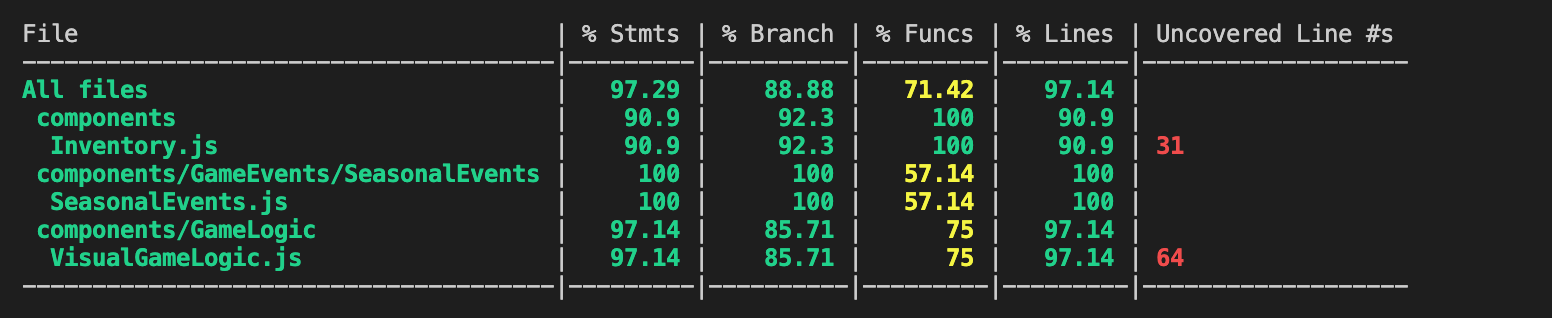
\includegraphics[width=\textwidth]{./Coverage.png}
\caption{Test Coverage for Unit Testing Inventory, Game Logic, and Events}
\label{FigCC1}
\end{figure}

\begin{figure}[H]
\centering
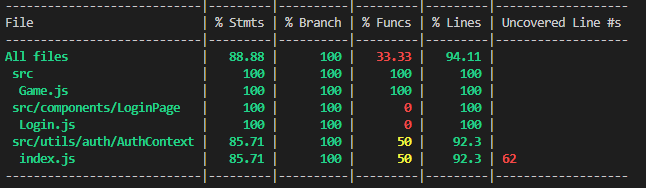
\includegraphics[width=\textwidth]{./Coverage2.png}
\caption{Test Coverage for Testing Accounts and Authentication}
\label{FigCC2}
\end{figure}

\bibliographystyle{plainnat}
\bibliography{../../refs/References}

\newpage{}
\section{Appendix}
\subsection{Symbolic Parameters}

The definition of the test cases will call for SYMBOLIC\_CONSTANTS.
Their values are defined in this section for easy maintenance.

\begin{table}[h]
\caption{\bf Symbolic Parameter Table}
\resizebox{6in}{!}{\begin{tabular}{|l|p{0.5\linewidth}|p{0.3\linewidth}|}
\hline
\multicolumn{1}{|l}{\bfseries Symbolic Parameter} & \multicolumn{1}{|l|}{\bfseries Description} & \multicolumn{1}{l|}{\bfseries Value}\\
\hline
NEW\_ACCOUNT\_STATE & The initial state of a new account & Turn 0, 9 tiles of land owned, USER\_MONEY \\
\hline
 SCREEN\_RESOLUTIONS & The list of screen resolutions that are supported by the user interface; given as a width and height & 1920 pixels x 1080 pixels, 1366 pixels x 768, pixels, 1536 pixels x 864 pixels, 1440 pixels x 900 pixels, 1280 pixels x 720 pixels\\
 % link for most common screen resolution sizes https://gs.statcounter.com/screen-resolution-stats/desktop/canada
\hline
MIN\_TURNS & The minimum amount of turns played needed for a study participant to be a significant data point & 12 turns\\
\hline
CONSULTANT\_PRICE & The default price to purchase a consultant's advice & \$150\\
\hline
ITEM\_PRICE & The default price of a item & \$150\\
\hline
USER\_MONEY & The money a user has & USER\_MONEY\\
\hline
EXPECTED\_SURVEY\_RATING & The expected survey rating to result as a pass & 4\\
\hline
MAX\_RESPONSE\_TIME & The maximum time allowed for the system to respond by & 5 seconds\\
\hline
MAX\_INTERFACE\_UPDATE\_TIME & The maximum time allowed for the interface to respond by & 1 second\\
\hline
\end{tabular}}
\end{table}

\subsection{Usability Survey Questions}

\begin{table}[h]
\resizebox{5.5in}{!}{\begin{tabular}{|lllllll|}
\hline
\multicolumn{7}{|c|}{\textbf{User Experience Survery}}\\
\multicolumn{7}{|l|}{}                                \\ \hline
\multicolumn{7}{|l|}{\textit{The following survey will be completed upon playing the game after 20 minutes}}  
                \\ \hline
\multicolumn{7}{|l|}{\textbf{Look and Feel}} \\
\multicolumn{7}{|l|}{}   
\\ \hline
\multicolumn{1}{|l|}{Minimalistic Design}    & \multicolumn{1}{l|}{0} & \multicolumn{1}{l|}{1} & \multicolumn{1}{l|}{2} & \multicolumn{1}{l|}{3} & \multicolumn{1}{l|}{4} & 5 \\ \hline
\multicolumn{1}{|l|}{}                       & \multicolumn{6}{c|}{{[}0 = too much clutter of elements, 5 = no clutter and minimal feel{]}}                                   \\ \hline
\multicolumn{1}{|l|}{Consistent Color Theme} & \multicolumn{1}{l|}{0} & \multicolumn{1}{l|}{1} & \multicolumn{1}{l|}{2} & \multicolumn{1}{l|}{3} & \multicolumn{1}{l|}{4} & 5\\ \hline
\multicolumn{1}{|l|}{}                       & \multicolumn{6}{c|}{{[}0 = inconsistent color theme, 5 = consistent color theme{]}}                                            \\ \hline
\multicolumn{1}{|l|}{Engaging Audio}         & \multicolumn{1}{l|}{0} & \multicolumn{1}{l|}{1} & \multicolumn{1}{l|}{2} & \multicolumn{1}{l|}{3} & \multicolumn{1}{l|}{4} & 5 \\ \hline
\multicolumn{1}{|l|}{}                       & \multicolumn{6}{c|}{{[}0 = audio is terrible to listen to, 5 = audio is enjoyable to listen to{]}}                             \\ \hline
\multicolumn{1}{|l|}{Engaging Graphics}      & \multicolumn{1}{l|}{0} & \multicolumn{1}{l|}{1} & \multicolumn{1}{l|}{2} & \multicolumn{1}{l|}{3} & \multicolumn{1}{l|}{4} & 5 \\ \hline
\multicolumn{1}{|l|}{}                       & \multicolumn{6}{c|}{{[}0 = graphics are not pleasing, 5 = graphics are pleasing and comfortable{]}}                            \\ \hline

\multicolumn{7}{|l|}{\textbf{Usability}}  \\
\multicolumn{7}{|l|}{}  
\\ \hline
\multicolumn{1}{|l|}{Age Group}      & \multicolumn{1}{l|}{0} & \multicolumn{1}{l|}{1} & \multicolumn{1}{l}{} & \multicolumn{1}{l}{} & \multicolumn{1}{l}{} &  \\ \hline
\multicolumn{1}{|l|}{}                       & \multicolumn{6}{c|}{{[}0 = age less than 18, 1 = age is 18 or above{]}}                            \\ \hline
\multicolumn{1}{|l|}{Easy to understand}      & \multicolumn{1}{l|}{0} & \multicolumn{1}{l|}{1} & \multicolumn{1}{l|}{2} & \multicolumn{1}{l|}{3} & \multicolumn{1}{l|}{4} & 5 \\ \hline
\multicolumn{1}{|l|}{}                       & \multicolumn{6}{c|}{{[}0 = hard to understand, 5 = easy enough to understand{]}}                            \\ \hline
\end{tabular}}
\end{table}

\newpage{}
\section*{Appendix --- Reflection}

The information in this section will be used to evaluate the team members on the
graduate attribute of Reflection.  Please answer the following question:

\begin{enumerate}
  \item In what ways was the Verification and Validation (VnV) Plan different
  from the activities that were actually conducted for VnV?  If there were
  differences, what changes required modification in the plan?  Why did
  these changes occur?  Would you be able to anticipate these changes in future
  projects?  If there weren't any differences, how was your team able to clearly
  predict a feasible amount of effort and the right tasks needed to build the
  evidence that demonstrates the required quality?  (It is expected that most
  teams will have had to deviate from their original VnV Plan.)
\end{enumerate}

One way the VnV Plan was different from what we actually conducted was that some tests were added and some tests were removed due to requirements changing. For example in the VnV Plan, we had planned to allow users to buy buildings. However, this functionality was removed later on in development as the team didn't see a need for them in terms of game mechanics. With this removal, the tests associated with this functionality were removed as well. Another change was with where we would store game logic. In the VnV Plan, we first had it such that clients would have to make requests to the server to do any game action such as buying or planting seeds, harvesting or selling crops, etc. The architecture now is that the game logic is stored and handled client side, and so performance testing of the game logic API requests was no longer needed.

These changes mostly arose from the fact that the team did not fully plan and discuss all game mechanics and how they would be intertwined with each other. They were mostly discussed in a vacuum rather than what role they would play in the encompassing game loop.

For future projects, we will further emphasize thorough planning of the entire product. This can be done by a number of visualization or planning methods such as sketches, storyboards, paper prototypes, or any other low-fidelity prototype. More communication with the client such as more meetings would also help iron out all the details of the project and reduce the number of changes or clarifications later on in development. However, even with all of this, there is still no guarantee that all possible changes are anticipated, which further highlights how important it is to minimize these possibilities.

\end{document}